\documentclass[landscape,a3,final,24pt]{issposter}

% If you encounter errors like "No room for a new ...", use etex (needs
% to be the first package. This happens, if too many registers are used
% because of too many packages or too many complex packages (like e.g. 
% tikz, pstricks and longtable). etex extends the number of registers.
% etex has to be the first package to be loaded!
% \usepackage{etex}

\usepackage[latin1]{inputenc}
\usepackage{multicol}
\usepackage{graphicx}
\usepackage[ngerman]{babel}
\usepackage{amsmath}
\usepackage{amsfonts}
\usepackage{amssymb}
\usepackage{booktabs} 

% If you want to use latex, dvips and ps2pdf, use hyperref to get correct
% page sizes. With hyperref, you won't have to specify them on the command
% line.
% \usepackage[pdfpagemode=UseNone,dvips,pdfborder={0 0 0}]{hyperref}

% \usepackage{tikz} % nice graphics, also used for the fancy boxes

% \usepackage{pstricks,pst-plot,pst-node} % nice graphics with PS
% \psset{unit=3mm,nodesep=1.5,linewidth=.3}
% Use auto-pst-pdf, to use PSTricks with pdflatex. In this case,
% you have to add --shell-escape to your pdflatex command line.
% \usepackage{auto-pst-pdf}

% Set the font sizes. Change these, if you want to change only one or two.
% Use the font size options of the document class (14pt, 17pt, 20pt, 15pt, 30pt, 36pt),
% if you want to change all the sizes at once.
\renewcommand{\titlesize}{\Huge}
\renewcommand{\sectionsize} {\Large}
\renewcommand{\authorsize}{\Large}
\renewcommand{\instsize}{\large}
\renewcommand{\normalsize}{\fontsize{8.5}{9}\selectfont}

% Insert your data
\title{\MakeUppercase{Human Activity Recognition}}
\author{Yitian Shi and Jonas Vogt}
\institute{Institute of Signal Processing and System Theory, University of Stuttgart, Germany}
\conference{\normalsize \textbf{Deep Learning Lab 2022}, February 4, Stuttgart, Germany }

% -----------------------------------------------------------------------------
\begin{document}
\maketitle

% Justified text sometimes looks strange in narrow columns
\raggedright

\begin{multicols}{3}
\section{Datasets Overview and Preprocess }
Besides the data preprocessing pipeline mentioned in the script, there are still some important data handling techniques that deal with the different characteristics and difficulties of each dataset.
\begin{itemize}\item HAPT\end{itemize}
\begin{figure}
\centering
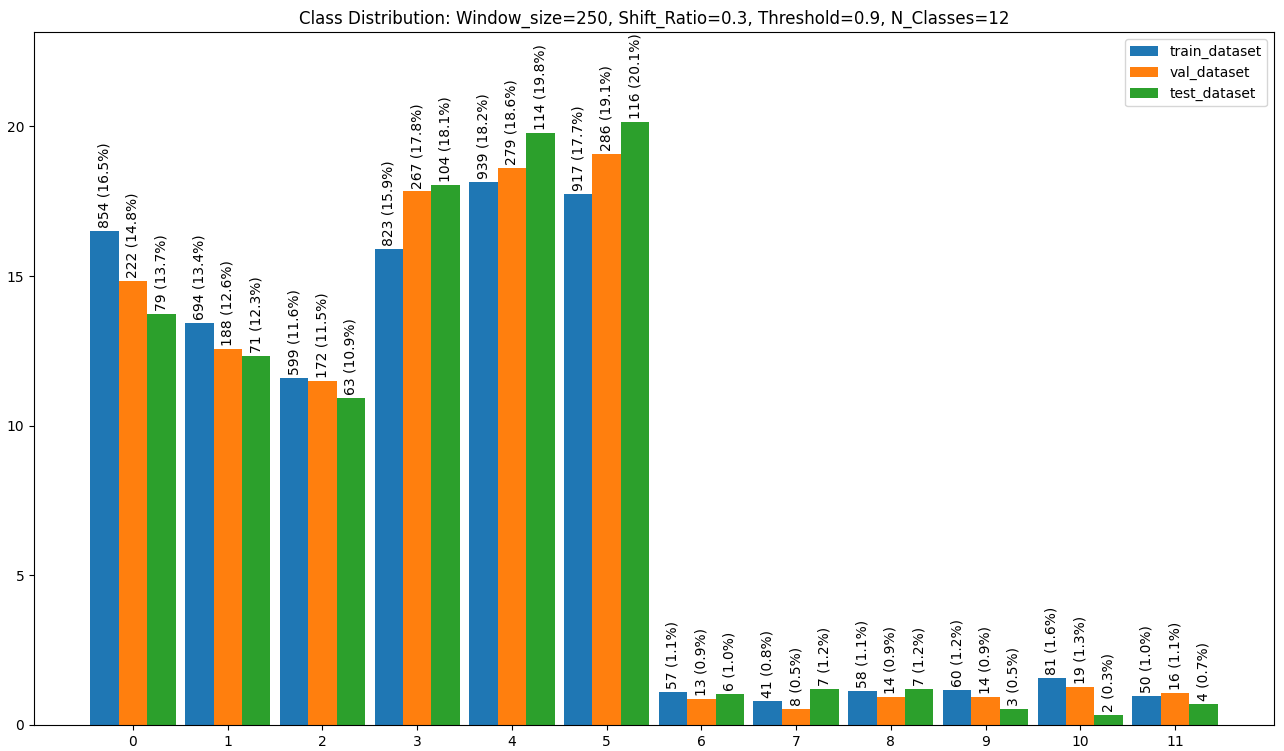
\includegraphics[scale=0.27]{Pictures/HAPT_class_distribution.png}
%\caption{sample: class distribution}
\end{figure}

According to the data statistics, the dataset contains highly imbalanced data between continuous and transitional classes (such as SIT\_TO\_STAND, STAND\_TO\_SIT, etc.). These activities are prioritized while using the sliding window techniques in such a way, that a windows will be labeld by the transitional class when this activity is in between (framed by) two continuous activities.

\begin{figure}
\centering
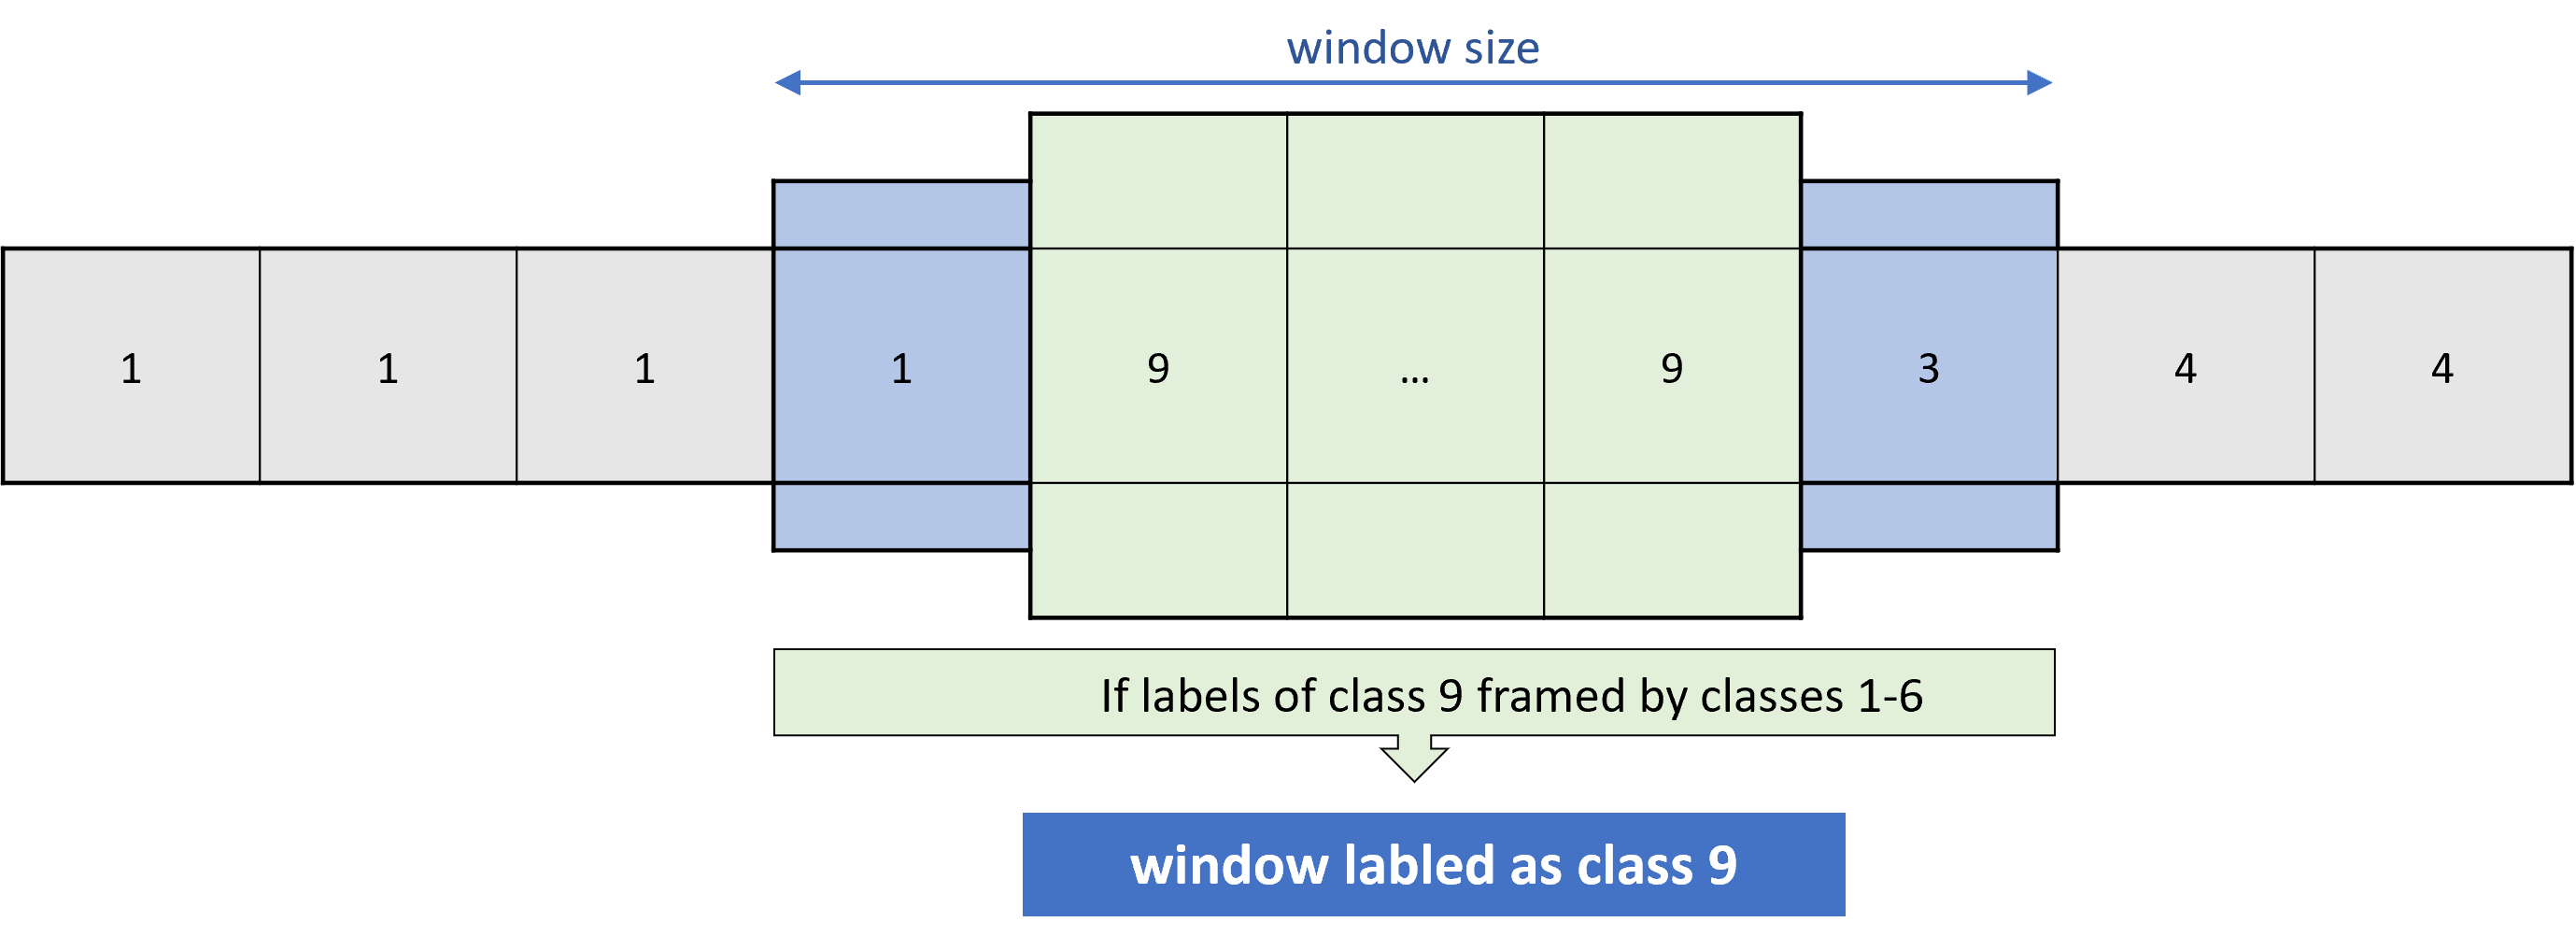
\includegraphics[scale=0.55]{Pictures/sliding Window_prio.png}
%\caption{sample: running}
\end{figure}

\begin{itemize}
\item HAR realworld2016\end{itemize}

\begin{figure}
\centering
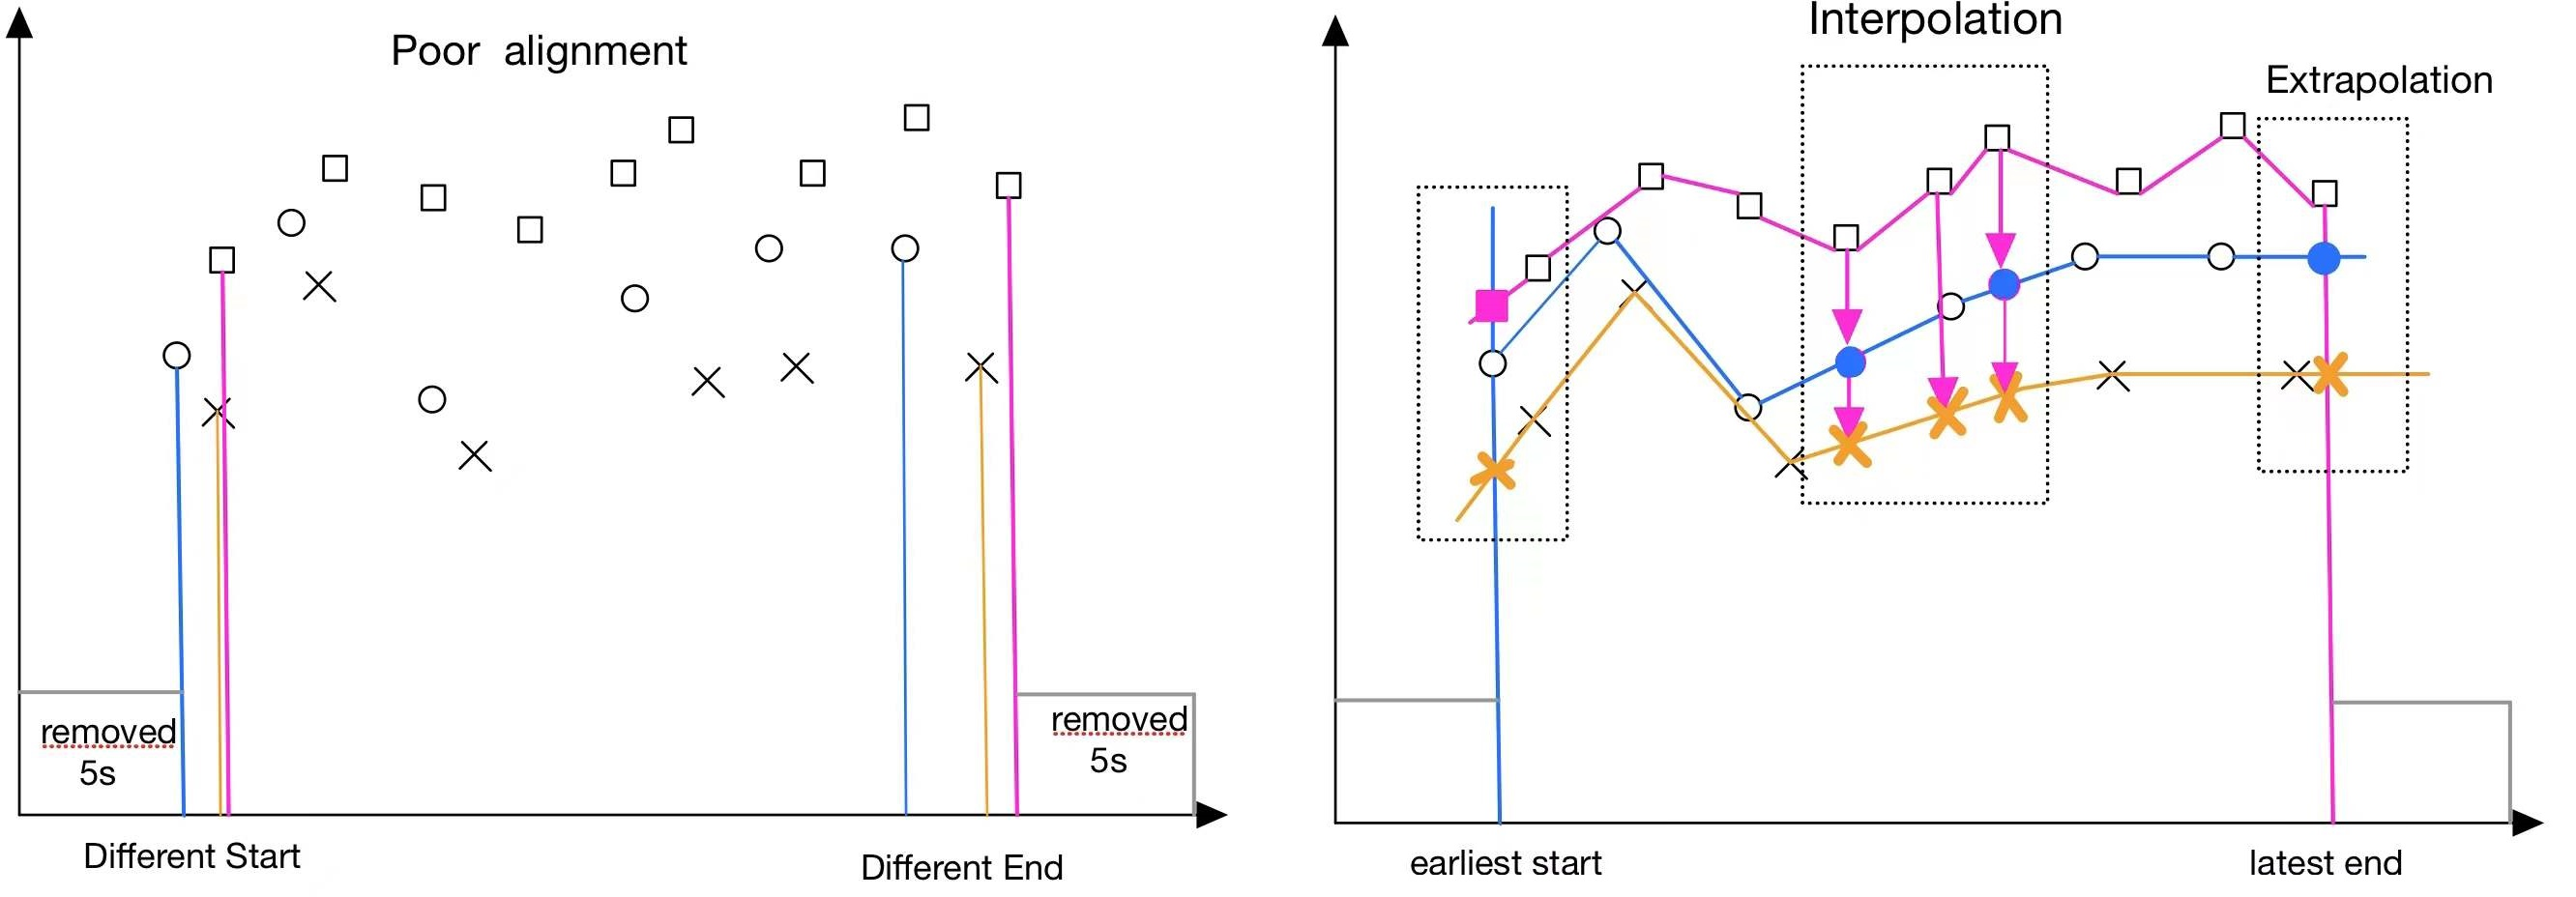
\includegraphics[scale=0.175]{Pictures/Interpolation_example.jpg}
\label{sample running}
\end{figure}

Because of the slight differences of recording time in several milliseconds, the data is not perfectly aligned.By nearest inter/extrapolation of all the data on the same discrete-time range will solve this problem under the assumption, that the data doesn't change itself in between 20ms, which corresponds to the smallest sampling period.

\vfill\null
\columnbreak


\section{Models \& Results}
\begin{itemize}\item HAPT\end{itemize}

Besides traditional RNN and LSTM architectures, we've also applied the Transformer encoder structure as the backbone with a normal classification head. We have the following configurations compared to the model structure from the base model in the paper 'Attention is all you need':

\hspace*{\fill} \\

\begin{tabular}{cccccc}
\toprule
Model	&layers&d\_model&d\_feed\_forward&num\_head&d\_key/value\\
\midrule
Base model&	6&	512&	2048&	8&	64\\
Our model	&1&	32&	128&	4&	8\\
\bottomrule
\end{tabular}

\hspace*{\fill} \\
\hspace*{\fill} \\
The best results we've achieved are as follows:
\hspace*{\fill} \\
\hspace*{\fill} \\


\begin{tabular}{cccc}

   \toprule
   Architecture  & Window size &Dropout rate& Balanced test accuracy \\
   \midrule
   LSTM 13&250 &0.4& 86.92\% \\
   LSTM 10&300 &0.2&88.90\% \\
   GRU 10&300 &0.2&  84.44\% \\
   
   Stacked LSTM (11,11)&250&0.1& 91.40\% \\
   Stacked GRU (11,11)&300&0.1& 77.91\% \\
   Stacked LSTM (15,12)&250&0.3 & 88.50\% \\
   Stacked LSTM (8,11)&250&0.5 & 84.50\% \\
   Transformer encoder & 300&&82.28\%  \\
   Soft-Voting &250& & \textbf{91.64\%}\\
   \bottomrule
\
\end{tabular}

\begin{figure}[htbp]
\centering
\subfigure[Transformer encoder]{
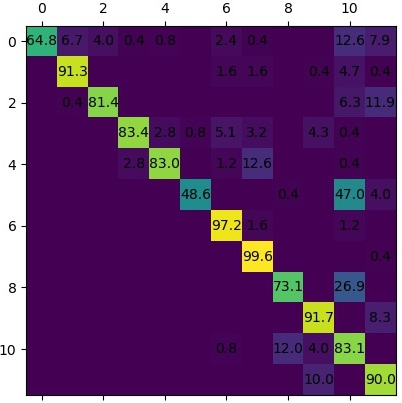
\includegraphics[scale=0.48]{Pictures/transformer_encoder.jpg}
%\caption{fig1}
}
\quad
\subfigure[Soft voting]{
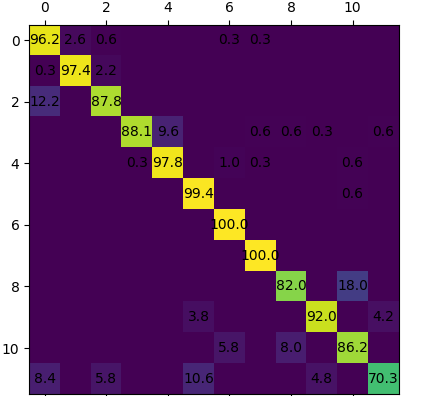
\includegraphics[scale=0.47]{Pictures/soft_voting_result.png}
%\caption{fig2}
}
\caption{Confusion matrices examples}
\end{figure}

 Hyperparamter tuning with Weights\&Biases:
\hspace*{\fill} \\
\hspace*{\fill} \\

\begin{center}
\begin{tabular}{cccc}
   \toprule
   \textbf{Hyperparameter}  & Window size &Shift-Ratio&  Labeling-Threshold \\
   \midrule
   \textbf{value}&250 &0.3&0.9 \\
   \bottomrule
\end{tabular}
\begin{figure}
\centering
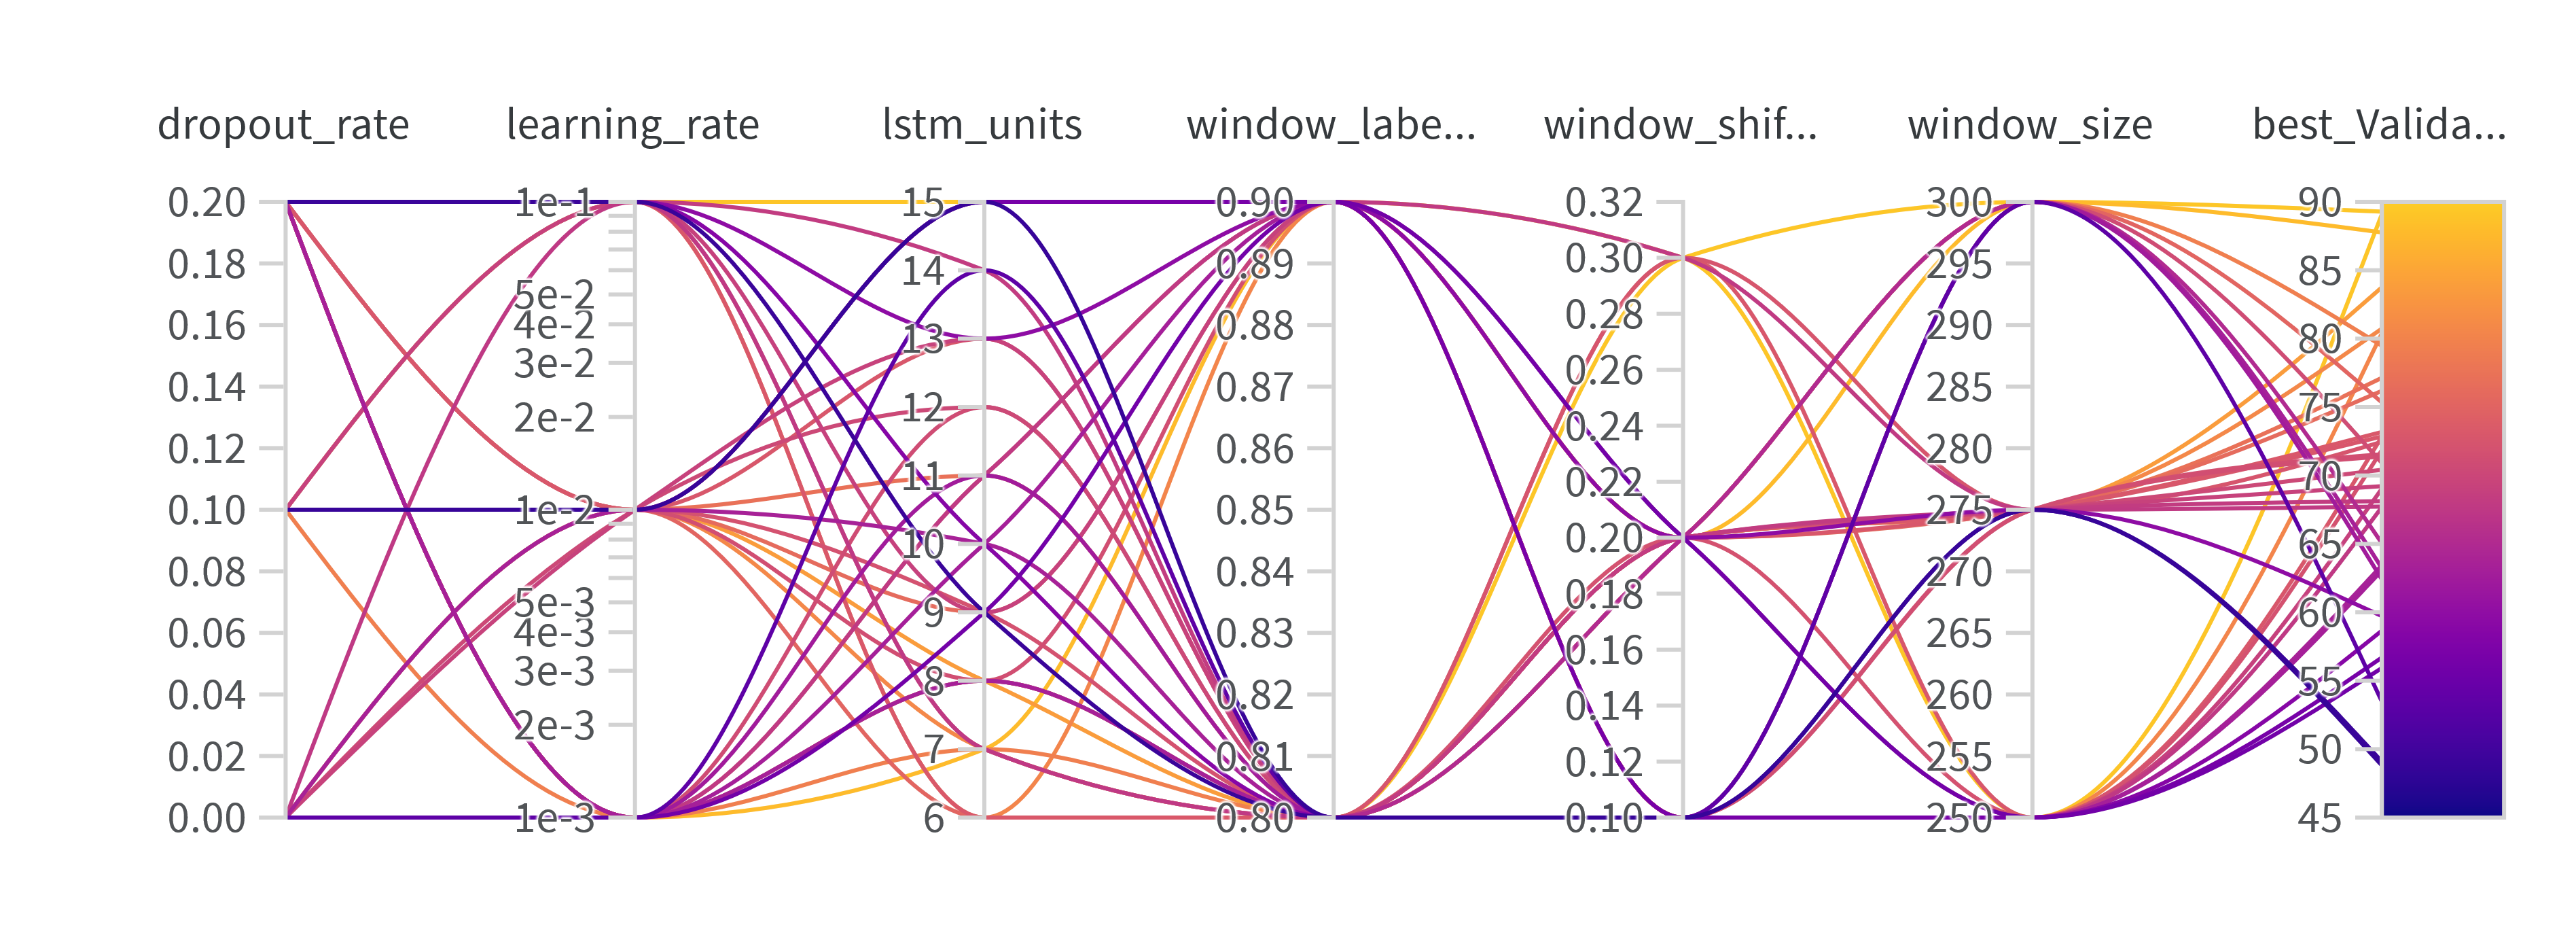
\includegraphics[width=\linewidth,keepaspectratio]{Pictures/wandb_sweep.png}
\end{figure}
\end{center}

\columnbreak
\begin{itemize}
\item HAR realworld2016\end{itemize}
We've tried different model architectures on different sensor positions. Some positions can present good accuracies on a specific position (one against others)
\begin{center}
\begin{tabular}{ccc}
   \toprule
  Sensor position& Architecture  &  Balanced test accuracy \\
  \midrule
  upperarm &stacked LSTM (10,10) &83.42\% \\
   chest &LSTM 10 &82.76\% \\
   shin &stacked LSTM (10,10)&81.84\% \\
   waist &stacked LSTM (10,10)&75.44\% \\
   forearm &stacked LSTM (10,10)& 73.03\% \\
  head &stacked LSTM (10,10)&67.32\%  \\
   \bottomrule
\end{tabular}
\end{center}
\begin{figure}[htbp]
\centering
\subfigure[upperarm]{
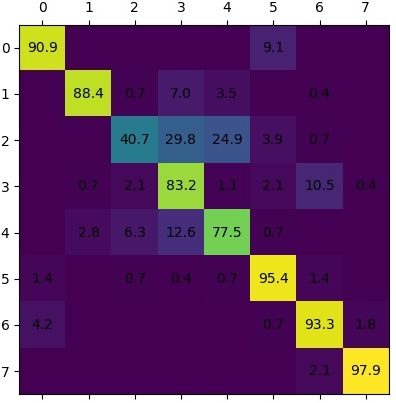
\includegraphics[scale=0.5]{Pictures/upperarm.jpg}
%\caption{fig1}
}
\quad
\subfigure[chest]{
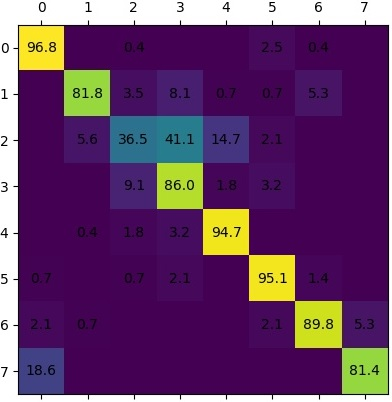
\includegraphics[scale=0.5]{Pictures/chest.jpg}
%\caption{fig2}
}
\caption{Confusion matrices examples}
\end{figure}

Meanwhile, we've also discovered the situation, that some of the sensor data give a big difference between the best validation and test accuracy caused by different distributions of both datasets. One reason we assume is the variety of human physical characteristics which influence their activity behaviors. These results comparisons are as follows:
\begin{center}
\begin{tabular}{ccccc}
   \toprule
  Position& Architecture  & Validation&Test&accuracy difference \\
  \midrule
  upperarm	&stacked LSTM (10,10)	&49.40\%	&83.42\%	&-34.02\%\\
waist	&stacked LSTM (10,10)	&52.99\%	&75.44\%	&-22.45\%\\
thigh	&LSTM 11	&76.69\%	&56.32\%	&20.37\%\\
   \bottomrule
\end{tabular}
\end{center}
\section{Android Application}
Last but not least we've developed an android application to record the realtime sensor data and make predictions using Tensorflow Lite model.After each 6 seconds (300 samples with 20ms sampling period) the probabilities of each classes will be refreshed. This module is still under development because of some adaptation issues.

\begin{figure}
\centering
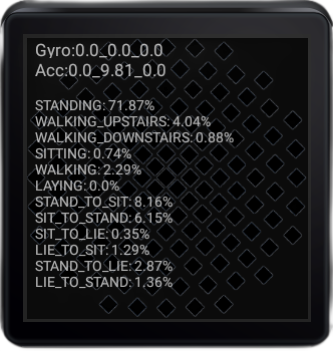
\includegraphics[scale=0.5]{Pictures/Android_example.png}
%\caption{sample: running}
\end{figure}

\end{multicols}

\end{document}






